\documentclass[12pt, a4paper, oneside]{ctexart}
\usepackage{amsmath, amsthm, amssymb, bm, graphicx, hyperref, geometry, mathrsfs,color}

\title{\huge\textbf{集合与实数集}}
\author{luojunxun}
\date{\today}
\linespread{2}%行间距
\geometry{left=2cm,right=2cm,top=2cm,bottom=2cm}%设置页面
\CTEXsetup[format={\Large\bfseries}]{section}%section左对齐

%定义环境
\newenvironment{Def}[1][def-name]{\par\noindent{\textit{(#1):}\small}}{\\\par}
\newenvironment{theorem}[1][Theorem-name]{\par\noindent \textbf{Theorem #1:}\textit}{\\\par}
\newenvironment{lemma}[1][lemma-name]{\par\noindent \textbf{Lemma #1:}\textbf}{\\\par}
\renewenvironment{proof}{\par\noindent{\textit{Proof:}\small}}{\\\par}
\newenvironment{example}[1][example-name]{\par{\textbf{Example:}}}{\\\par}
\newenvironment{say}{\center{\textit{summary:}}}{\\\par}
\newenvironment{note}[1][note-name]{\par\textit{#1:}}{\\\par}


\begin{document}
\maketitle

\section*{映射}
\Def[映射]{$X,Y$是两个集合,在其中定义了一个关系$f$,使得$\forall x\in X,\exists ! y\in Y,s.t.x\to y$\\
y是x在f下的像,x是y在f下的原像\\
满射:$\forall y\in Y,\exists x\in X,s.t.y=f(x)$称f是一个满射,或者完全映射\\
单射:$\forall x_1\neq x_2,f(x_1)\neq f(x_2)$称f是一个单射(或者一一映射,这里和数分的说法有矛盾,数分的一一映射指的是这里的双射)\\
双射:既是单射又是满射;\\
}

$A\subset X.B\subset Y$有:\\
1.$f(A)=\{f(x)|x\in A\}\subset Y$称为A在f下的像\\
2.$f^{-1}(B)=\{x\in X|f(x)\in B\}\subset X$称为B在f下的原像

映射性质:复合映射,复合映射满足交换律

\theorem[定理]{
    $f:X\to Y,\Gamma$是指标集\\
    $1.f(\bigcup\limits_{\gamma\in\Gamma}A_\gamma)=\bigcup\limits_{\gamma\in\Gamma}f(A_\gamma)\quad
    {\color{red}{f(\bigcap\limits_{\gamma\in\Gamma}A_\gamma)\subset\bigcap\limits_{\gamma\in\Gamma}f(A_\gamma)}}\\
    2.B_1\subset B_2\subset Y\Rightarrow f^{-1}(B_1)\subset f^{-1}(B_2)\\
    3.f^{-1}(\bigcup\limits_{\beta\in\Gamma}B_\gamma)=\bigcup\limits_{\beta\in\Gamma}f(B_\gamma)\\
    4.f^{-1}(B^c)=(f^{-1}(B))^c$
}
\begin{proof}[1的证明]
    $y\in f(\bigcup\limits_{\gamma\in\Gamma}A_\gamma)\iff \exists x\in \bigcup\limits_{\gamma\in\Gamma}A_\gamma
    ,s.t.y=f(x)\iff \exists {\gamma_0}\in\Gamma ,s.t. x\in A_{\gamma_0}\iff y=f(x)\in f(A_{\gamma_0})\subset 
    \bigcup\limits_{\gamma\in\Gamma}f(A_\gamma)$得证\\
    $y\in f(\bigcap\limits_{\gamma\in\Gamma}A_\gamma)\iff \exists x\in \bigcap\limits_{\gamma\in\Gamma}A_\gamma
    ,s.t.y=f(x)\Rightarrow \quad\forall \gamma\in\Gamma ,\exists x_\gamma\in A_\gamma s.t.y=f(x_\gamma)\Rightarrow 
    \forall \gamma\in\Gamma ,y\in f(A_\gamma)\Rightarrow y\in \bigcap\limits_{\gamma\in\Gamma}f(A_\gamma)$
    \\(这里的不等号主要是因为f不一定是单射,第一个推出符号拉回来的时候$A_\gamma$可以没有公共的$x_\gamma$)
    \\其他的证明是平凡的
\end{proof}



\section*{特征函数}
\Def[$\mathcal{X}_A(x)$]{
    $A\subset X:\mathcal{X}_A(x)=
        \begin{cases}
            1\quad x\in A\\
            0\quad x\in X-A
        \end{cases}$
}

\theorem[性质]{\center{
    1.集合相等当且仅当他们的特征函数相等\\
    2.$A\subset B \to\mathcal{X}_A(x)\leq \mathcal{X}_B(x)$\\
    3.$\mathcal{X}_{A\cap{B}}(x)=\mathcal{X}_A(x)\mathcal{X}_B(x)$\\
    4.$\mathcal{X}_{A\cup{B}}(x)=\mathcal{X}_A(x)+\mathcal{X}_B(x)-\mathcal{X}_{A\cap{B}}(x)$\\
    5.$\mathcal{X}_{A-B}(x)=\mathcal{X}_A(x)(1-\mathcal{X}_B(x))$\\
    6.$\mathcal{X}_{A\Delta B}(x)=|\mathcal{X}_A(x)-\mathcal{X}_B(x)|$\\
    7.$\mathcal{X}_{\varlimsup\limits_{n\to\infty}A_n}(x)=\varlimsup\limits_{n\to\infty}\mathcal{X}_{A_n}(x)$\\
    8.$\mathcal{X}_{\varliminf\limits_{n\to\infty}A_n}(x)=\varliminf\limits_{n\to\infty}\mathcal{X}_{A_n}(x)$\\
证明在最后手写}}
\\\\\\

\section*{集合的等价,基数(势)}

\Def[集合等价]{A和B等价即A,B之间存在一个双射;称A,B有相同的基数,用$A\sim B$表示}

\theorem[集族的并的等价]{
    $\{A_\lambda|\lambda\in\Lambda\},\{B_\lambda|\lambda\in\Lambda\}$分别是两个元素两两不交的集族,如果
        $\forall \lambda\in\Lambda ,A_\lambda \sim B_\lambda\Rightarrow \bigcup\{A_\lambda|\lambda\in\Lambda\}\sim
        \bigcup \{B_\lambda|\lambda\in\Lambda\}$
}

\begin{proof}[集族并的等价]
    因为$\forall \lambda\in\Lambda,A_\lambda\sim B_\lambda$故$\exists f_\lambda$是$A_\lambda$到$B_\lambda$的双射,
    定义$f;s.t.f_{|A_\lambda}=f_\lambda$即可(这里用到了集族的元两两不交)
\end{proof}



\begin{figure}[p]

    \centerline{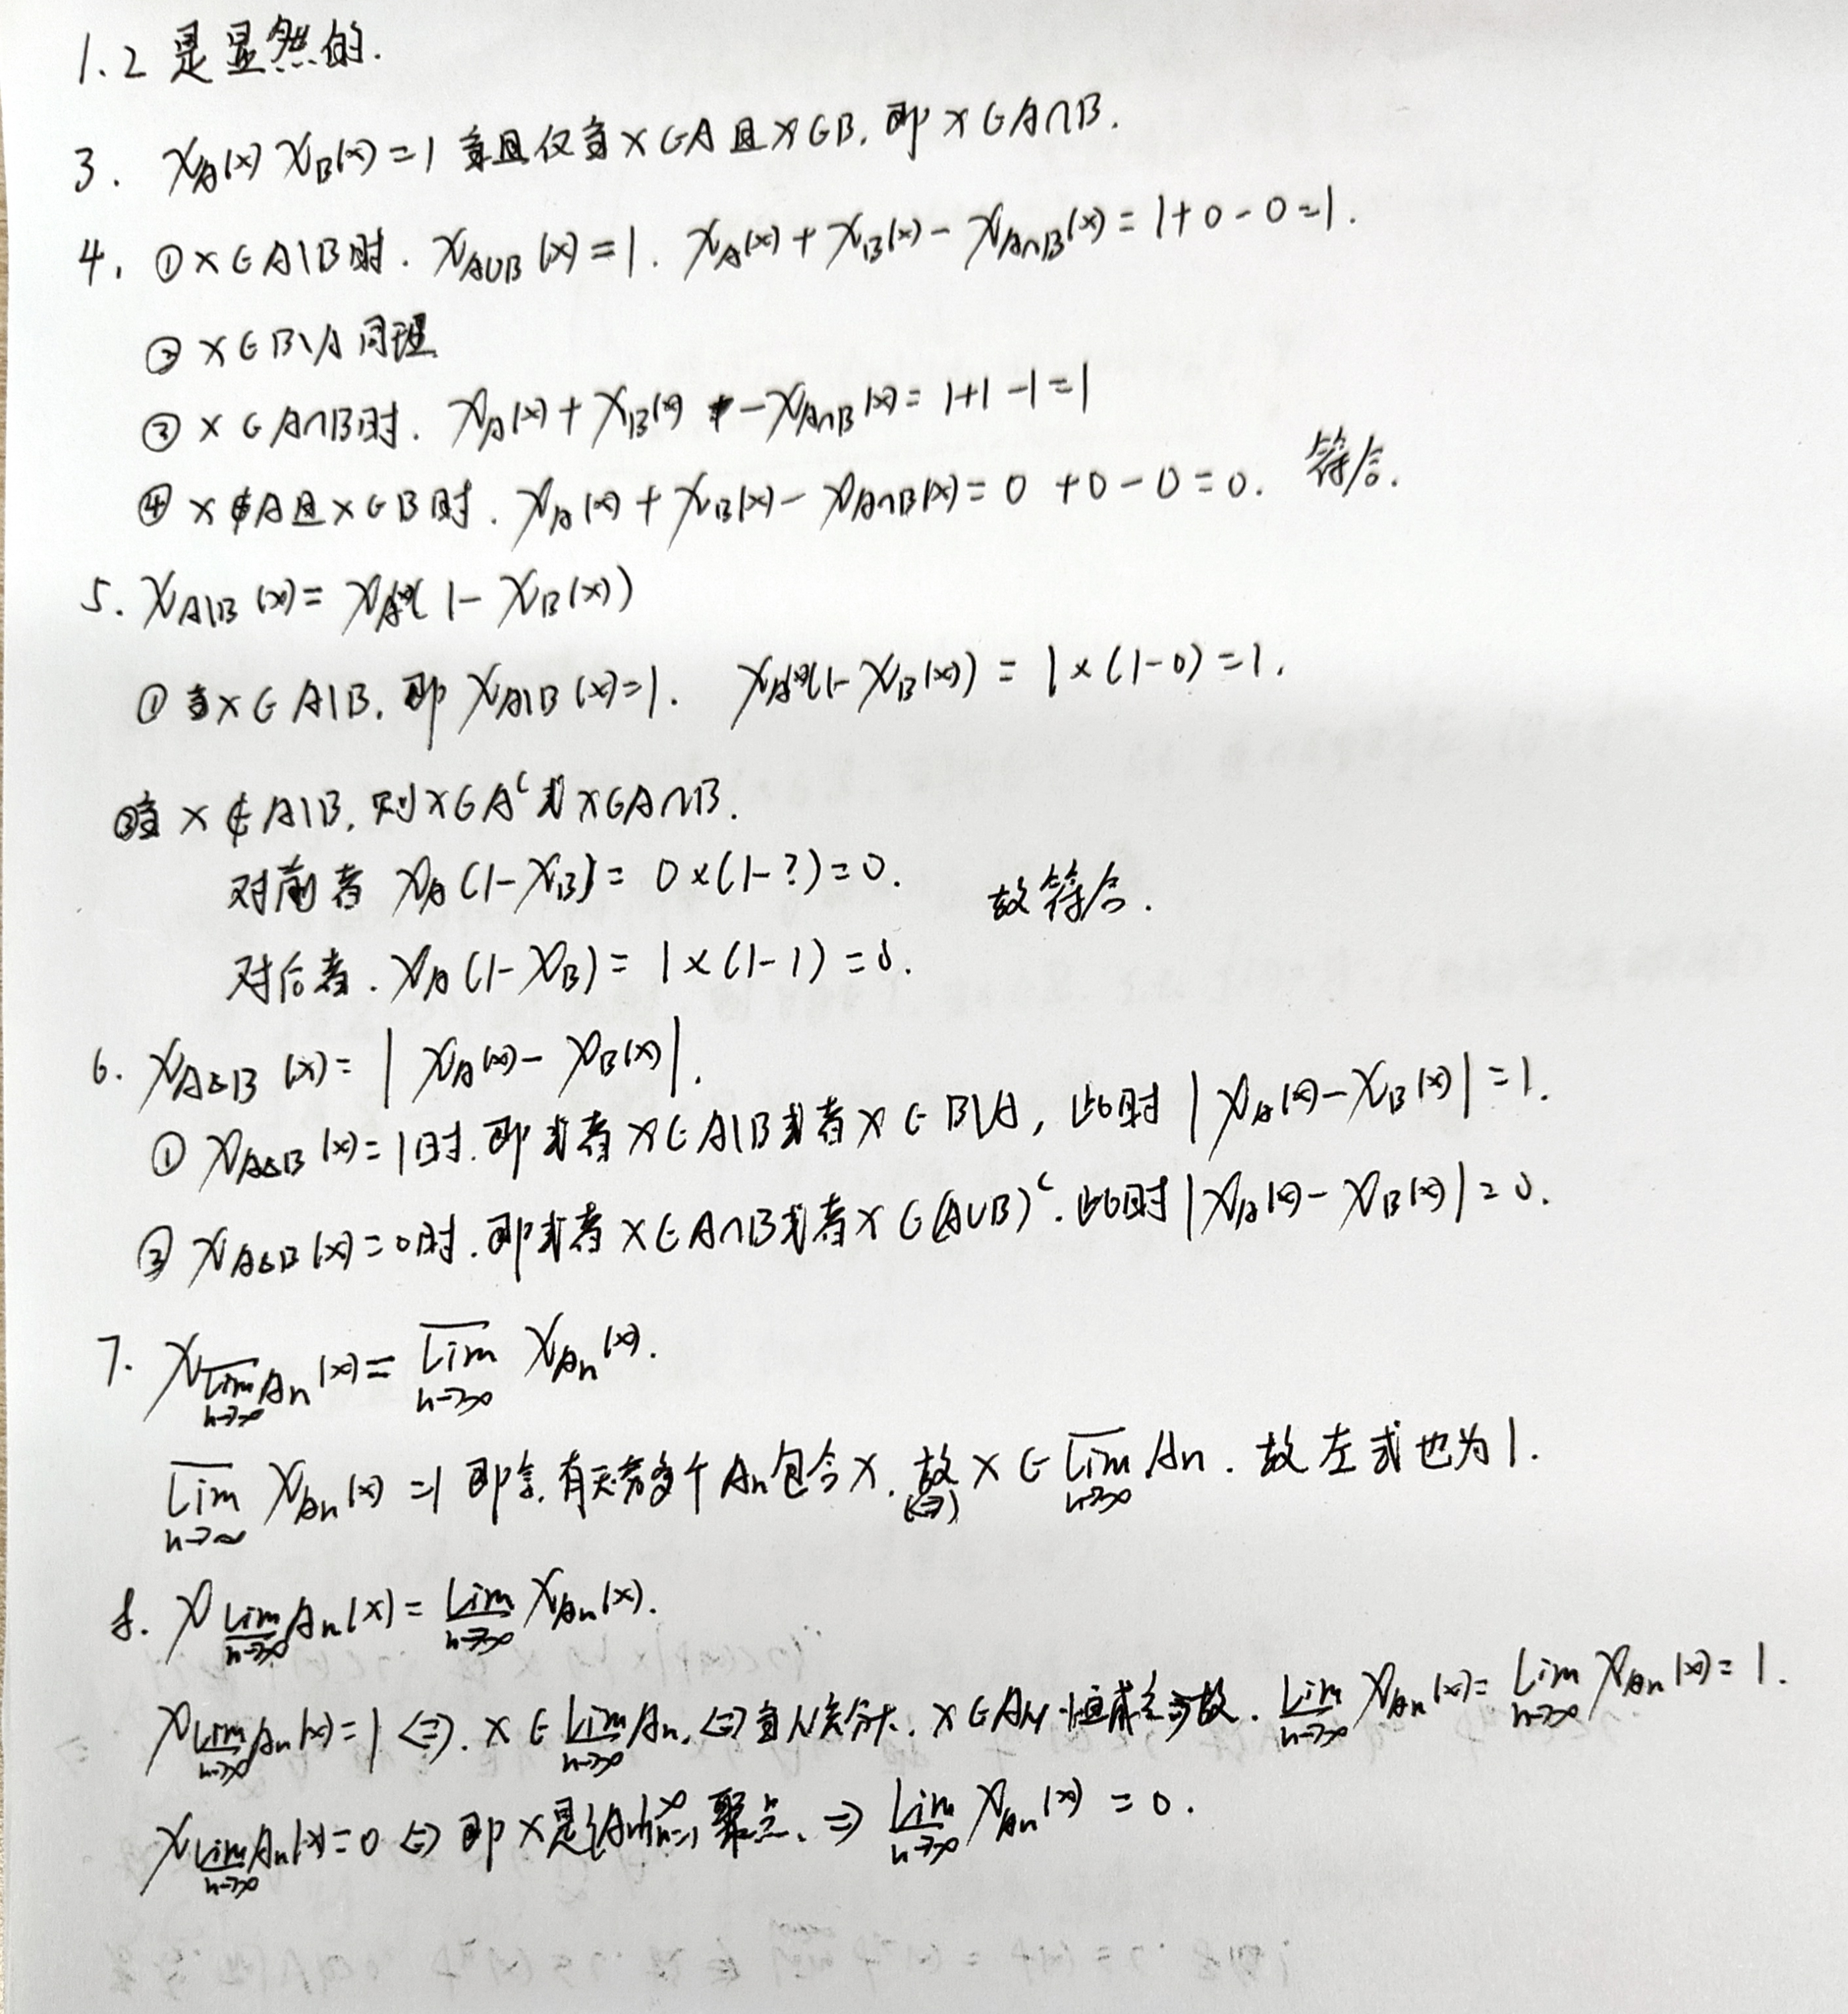
\includegraphics[width=1.2\linewidth,height=0.8\textheight]{proof.jpg}}
    \caption{证明}
    \label{figure}

\end{figure}























\end{document}